\section{Konsep Kriptografi Asimetris dan Kunci Publik}

Dalam kriptografi asimetris, setiap pihak memiliki \textbf{pasangan kunci}: kunci publik (dapat dibagikan) dan kunci privat (rahasia). Enkripsi dengan kunci publik hanya dapat didekripsi dengan kunci privat yang sesuai. Sistem ini merevolusi cara komunikasi aman dengan menghilangkan kebutuhan untuk berbagi kunci rahasia melalui kanal yang aman.

Kriptografi asimetris pertama kali dipublikasikan oleh Whitfield Diffie dan Martin Hellman pada tahun 1976, yang membuka era baru dalam keamanan komunikasi digital. Menurut Wikipedia, konsep ini sangat revolusioner karena memungkinkan dua pihak yang belum pernah bertemu untuk berkomunikasi secara aman melalui jaringan publik. Ide dasar ini kemudian diimplementasikan secara praktis oleh Rivest, Shamir, dan Adleman dalam algoritma RSA yang menjadi fondasi kriptografi modern.

\textbf{Skema dasar}: Alice mempublikasikan kunci publik. Bob mengenkripsi pesan dengan kunci publik Alice. Hanya Alice (yang memiliki kunci privat) yang dapat mendekripsi. Sistem ini bekerja berdasarkan fungsi satu arah (one-way function) yang mudah dihitung dalam satu arah tetapi sangat sulit dibalikkan tanpa informasi rahasia.

\textbf{Manfaat}: Tidak perlu pertukaran kunci rahasia di kanal terbuka. Kunci publik dapat didistribusikan melalui direktori atau sertifikat. Menurut sumber keamanan, kemampuan untuk mendistribusikan kunci publik secara terbuka memungkinkan skala komunikasi aman yang sangat besar, seperti yang terlihat dalam internet modern dengan jutaan transaksi per hari.

\textbf{Keterbatasan}: Lebih lambat dibanding simetris. Umumnya digunakan untuk pertukaran kunci atau tanda tangan, bukan enkripsi data besar. Menurut Wikipedia, operasi matematika yang diperlukan untuk RSA (eksponensial modular) jauh lebih lambat dibandingkan operasi simetris seperti AES, sehingga penggunaan RSA untuk enkripsi data besar secara langsung tidak praktis.

\subsection{RSA untuk Enkripsi dan Tanda Tangan}

RSA dapat dipakai untuk \textbf{enkripsi} (gunakan kunci publik penerima) maupun \textbf{tanda tangan digital} (gunakan kunci privat pengirim). Keduanya memakai operasi modular yang sama, tetapi \textbf{tujuan dan padding} berbeda. Untuk enkripsi, skema yang direkomendasikan adalah RSAES-OAEP; untuk tanda tangan, skema yang direkomendasikan adalah RSASSA-PSS \cite{rfc8017}.

RSA dikembangkan oleh Ron Rivest, Adi Shamir, dan Leonard Adleman di MIT pada tahun 1977. Menurut Wikipedia, algoritma ini ditemukan setelah percobaan panjang selama satu tahun, dengan Rivest menghabiskan semalaman untuk memformalkan ide setelah tidak bisa tidur. Nama RSA berasal dari inisial nama belakang ketiga penemu dalam urutan yang sama seperti publikasi ilmiah mereka.

Secara praktik, RSA lebih sering digunakan untuk \textbf{key transport} (mengamankan kunci simetris) dan \textbf{signature}. Enkripsi data besar langsung dengan RSA tidak efisien dan dibatasi ukuran pesan, sehingga skema hybrid jauh lebih umum di sistem nyata. Menurut sumber keamanan, RSA dengan padding yang tepat (seperti OAEP) dapat membuktikan keamanannya secara matematis, tetapi implementasi yang salah dapat menyebabkan kerentanan yang serius.

\subsection{Hybrid Encryption dan KEM-DEM}

Karena RSA lambat, praktik umum adalah \textbf{hybrid encryption}: RSA hanya dipakai untuk mengamankan kunci simetris, sedangkan data utama dienkripsi dengan AES. Pola ini sering disebut \textbf{KEM-DEM} (Key Encapsulation Mechanism - Data Encapsulation Mechanism) \cite{nist800_56b_r2}:
\begin{enumerate}
  \item Buat kunci simetris acak $K_s$.
  \item Enkripsi pesan dengan AES (mis. GCM) menggunakan $K_s$ sehingga menghasilkan ciphertext $C$.
  \item Enkripsi $K_s$ dengan RSA-OAEP sehingga menghasilkan $C_K$.
  \item Kirimkan $(C_K, C)$ kepada penerima.
\end{enumerate}
Penerima mendekripsi $C_K$ untuk memperoleh $K_s$, lalu mendekripsi $C$ dengan AES.

Hybrid encryption menjadi standar industri karena menggabungkan keunggulan kedua jenis kriptografi. Menurut sumber keamanan, KEM-DEM menyediakan keamanan yang dapat dibuktikan (provable security) dengan efisiensi operasional yang tinggi. Pendekatan ini memungkinkan enkripsi data berukuran besar dengan kecepatan AES sambil mempertahankan keamanan kunci publik RSA untuk pertukaran kunci.

\begin{figure}[htbp]
  \centering
  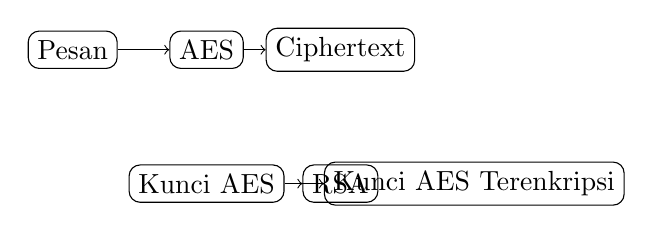
\begin{tikzpicture}[node distance=1.7cm]
    \node (msg) [draw, rounded corners] {Pesan};
    \node (aes) [draw, rounded corners, right of=msg] {AES};
    \node (ct) [draw, rounded corners, right of=aes] {Ciphertext};
    \node (key) [draw, rounded corners, below of=aes] {Kunci AES};
    \node (rsa) [draw, rounded corners, right of=key] {RSA};
    \node (ekey) [draw, rounded corners, right of=rsa] {Kunci AES Terenkripsi};
    \draw[->] (msg) -- (aes);
    \draw[->] (aes) -- (ct);
    \draw[->] (key) -- (rsa);
    \draw[->] (rsa) -- (ekey);
  \end{tikzpicture}
  \caption{Skema hybrid: RSA untuk kunci, AES untuk data.}
\end{figure}

\subsection{PKI dan Sertifikat}

Distribusi kunci publik membutuhkan \textbf{kepercayaan}. Dalam praktik, kunci publik dibungkus dalam sertifikat digital (PKI) agar identitas pemilik kunci dapat diverifikasi. Ini mencegah serangan \textit{man-in-the-middle} saat pertukaran kunci publik. Menurut Wikipedia, Public Key Infrastructure (PKI) menjadi fondasi untuk keamanan internet modern, memungkinkan verifikasi otomatis identitas digital.

PKI terdiri dari hierarki Certificate Authorities (CA) yang menerbitkan sertifikat digital setelah memverifikasi identitas pemohon. Menurut sumber keamanan, sertifikat mengandung kunci publik, informasi identitas, dan tanda tangan CA yang membuktikan keaslian. Sistem ini memungkinkan komunikasi aman antar pihak yang belum pernah bertemu, dengan kepercayaan yang didelegasikan melalui CA yang terpercaya.

\subsection{Validasi Kunci Publik dan Model Kepercayaan}

Saat menerima kunci publik (sertifikat), lakukan validasi dasar berikut:
\begin{itemize}
  \item Verifikasi rantai sertifikat sampai CA yang dipercaya.
  \item Cek masa berlaku, revocation (CRL/OCSP), dan penggunaan kunci (key usage).
  \item Pastikan identitas di sertifikat sesuai konteks (mis. domain atau identitas pengguna).
\end{itemize}
Tanpa validasi ini, enkripsi atau tanda tangan dapat mudah disusupi oleh kunci publik palsu.

Validasi sertifikat adalah langkah kritis dalam keamanan kriptografi asimetris. Menurut sumber keamanan, serangan man-in-the-middle berhasil ketika penyerang dapat menyisipkan kunci publik palsu yang dianggap sah oleh penerima. Proses validasi yang ketat, termasuk pemeriksaan Certificate Revocation Lists (CRL) dan Online Certificate Status Protocol (OCSP), sangat penting untuk mencegah penggunaan sertifikat yang telah dicabut.
